\subsection{WCF Service}

WCF(Windows Communication Foundation) – программный фреймворк, используемый для обмена данными между приложениями, входящий в состав .NET Framework. WCF сервисы призваны заменить и расширить ASMX веб сервисы. WCF сервисы предоставляют все те же возможности что и .NET веб сервисы и значительно расширяют их.

Простая и базовая разница заключается в том, что ASMX веб сервис предназначен для отправки и получения сообщений используя SOAP только через HTTP. В то же время WCF сервис может обмениваться сообщениями используя любой формат (SOAP является стандартным) через любой транспортный протокол (HTTP, TCP/IP, MSMQ, Named Pipes и т.д.).

ASMX веб сервисы могут быть размещены только в IIS, в то время как WCF сервис имеет следующие варианты хостинга:
\begin{itemize}
	\item IIS
	\item WAS (Windows Process Activation Services)
	\item Console Application
	\item Windows NT Services
	\item WCF provided Host
\end{itemize}

\begin{figure}[h!]
\centering
	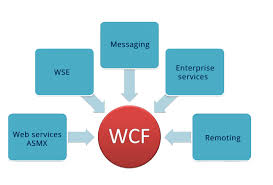
\includegraphics[scale=1]{wcf.jpg}
	\caption{Возможности WCF}
\end{figure}

Важной особенностью WCF сервисов в рамках проекта, является возможность осуществления потоковой передачи данных.